\chapter{微扰理论}\label{ch:b3:perturbation-theory}

只有寥寥数个量子问题可以精确求解：势阱、
振子、氢原子与二能级系统。其余问题——
原子置于场中、分子中变硬的化学键、
被邻近能级推动的能级——都是在可解骨架上
附加一个小项。\omterm{thm:b3:perturbation-theory:corrections}{微扰理论}的要旨，在于把这个附加项
视为一种修正，按其小量逐阶计算。
其一阶规则只是一个简单的平均；其二阶规则
解释了能级为何\emph{相互排斥}、为何每个原子都可以极化，
以及范德瓦尔斯吸引为何普遍存在；
其简并形式处理近乎相同的能级彻底重组的精细情形；
其含时形式——\omterm{thm:b3:perturbation-theory:golden}{费米黄金规则}——
是实验室中测得的每条吸收谱线、衰变率与
散射截面背后的方程。
作为附带的收获，本章最后将计算天空的颜色。

\section{小移动：非简并理论}

\begin{theorem}[微扰修正]\label{thm:b3:perturbation-theory:corrections}
\index{微扰理论}
设 $\hat H = \hat H_0 + \hat V$，其中 $\hat H_0$ 可精确求解，
即 $\hat H_0\ket n = E_n\ket n$，谱非简并，且 $\hat V$
为小量。则按 $\hat V$ 逐阶展开，
\[
E_n' = E_n + \bra n\hat V\ket n
 + \sum_{m \neq n}\frac{|\bra m\hat V\ket n|^2}{E_n - E_m}
 + \cdots
\]
且态矢获得混入项 $\ket{n'} = \ket n + \sum_{m\neq
n}\dfrac{\bra m\hat V\ket n}{E_n - E_m}\,\ket m + \cdots$
\emph{一阶}：能量移动即为微扰在
未微扰态中的平均值。\emph{二阶}：
与其他能级的耦合会使 $E_n$ \emph{远离}它们——
位于上方的每个 $m$ 把它往下推，位于下方的把它往上推——因此
基态的二阶移动总是负的。有效性要求混合
比例 $|\bra m\hat V\ket n/(E_n - E_m)|$ 必须很小。
\end{theorem}

\begin{proof}[部分证明]
将 $E' = E + \epsilon_1 + \epsilon_2 + \cdots$ 与 $\ket{\psi} =
\ket n + \ket{\psi_1} + \cdots$ 按 $\hat V$ 的幂次展开，代入
$(\hat H_0 + \hat V)\ket\psi = E'\ket\psi$，并按阶数比较。
将一阶方程投影到 $\bra n$ 上，即得 $\epsilon_1 =
\bra n\hat V\ket n$；投影到 $\bra m$（$m \neq n$）上则得混合系数；
将它们代入二阶方程，
再投影到 $\bra n$ 上即得 $\epsilon_2$。关于基态的符号结论：
每个分母 $E_0 - E_m$ 均为负，
而分子是平方项。
\end{proof}

\begin{proposition}[可精确求解的微扰]\label{prop:b3:perturbation-theory:oscillator-field}
电荷为 $q$ 的振子置于均匀场 $\mathcal E$ 中，
其 $\hat V = -q\mathcal E\hat x$。配方即可精确求解：
势能仍为同一抛物线，只是发生平移，所有能级整体降低
$q^2\mathcal E^2/2m\omega^2$。\omterm{thm:b3:perturbation-theory:corrections}{微扰理论}必须与之相符，
事实确实如此：一阶为零（$\langle\hat
x\rangle_n = 0$），二阶求和中 $\hat x$
仅使 $n$ 与 $n \pm 1$ 耦合，对每个能级恰好给出
$-q^2\mathcal E^2/2m\omega^2$。
（见\cref{exo:b3:perturbation-theory:2}）。一个可精确求解的例子，两种方法互相印证，
是方法所能获得的最好校准。
\end{proposition}

\begin{proof}
两个矩阵元及其分母给出
\[
\frac{|\bra{n+1}\hat x\ket{n}|^2}{-\hbar\omega}
 + \frac{|\bra{n-1}\hat x\ket n|^2}{+\hbar\omega}
 = \frac{\hbar}{2m\omega}\,\frac{-(n+1) + n}{\hbar\omega}
 = -\frac{1}{2m\omega^2} ;
\]
乘以 $q^2\mathcal E^2$。
\end{proof}

\begin{omfigure}
\begin{tikzpicture}
  \begin{axis}[omaxis, axis x line=bottom, axis y line=left,
    width=8.6cm, height=5.6cm, xmin=-1.6, xmax=1.6, ymin=-1.3, ymax=1.4,
    xlabel={耦合 $v$}, ylabel={能量},
    xlabel style={at={(axis description cs:0.5,-0.1)}, anchor=north},
    xtick=\empty, ytick=\empty, clip=false]
    \addplot[omDef, very thick, domain=-1.6:1.6, samples=90] {sqrt(0.09+x*x)};
    \addplot[omDef, very thick, domain=-1.6:1.6, samples=90] {-sqrt(0.09+x*x)};
    \addplot[gray, dashed, domain=-1.6:1.6] {0.3-0.35*0};
    \addplot[gray, dashed, domain=-1.6:1.6] {-0.3};
    \draw[gray, dashed] (axis cs:-1.6,0.3) -- (axis cs:1.6,0.3);
    \node[font=\scriptsize, anchor=west] at (axis cs:0.05,0.44) {间隙 $\ge$ 裸分裂};
    \draw[<->, omThm] (axis cs:0,0.3) -- (axis cs:0,-0.3);
    \node[omThm, font=\scriptsize, anchor=west] at (axis cs:0.05,-0.14) {最近处 $2|v|$};
    \node[omDef, font=\scriptsize, anchor=south] at (axis cs:-1.15,0.98) {上能级};
    \node[omDef, font=\scriptsize, anchor=north] at (axis cs:-1.15,-1.02) {下能级};
  \end{axis}
\end{tikzpicture}

{\small 能级排斥：两个耦合能级永不相交——随耦合
（或扫过裸能量的参数）变化时，精确能量
$\pm\sqrt{\Delta^2 + v^2}$ 彼此回避。二阶公式
即为这条双曲线的远翼；中心处的“避免交叉”
则是\omterm{thm:b3:perturbation-theory:corrections}{微扰理论}
让位于精确对角化的地方。}
\end{omfigure}

\section{能级简并时}

\begin{theorem}[简并微扰理论]\label{thm:b3:perturbation-theory:degenerate}
\index{简并微扰理论}
若 $E_n$ 简并，则上式会出现除以零的情况——
这时微扰可能使简并态彻底重组，
解决办法是顺势而为：\emph{将 $\hat V$ 限制在
简并子空间上对角化}。其\omterm{def:b3:quantum-formalism:observable}{本征值}即为一阶能量移动；
其本征态即为正确的零级态，
即微扰本身所选定的线性组合。
\end{theorem}
\admitted

\begin{example}[线性斯塔克效应]\label{ex:b3:perturbation-theory:stark}
\index{斯塔克效应}
氢原子的 $n = 2$ 能级包含简并的 $2s$ 态与 $2p$ 态。
在电场 $\mathcal E\vect e_z$ 中，$\hat V = e\mathcal E\hat z$
使 $2s$ 与 $2p_0$ 耦合，矩阵元为 $\bra{2s}\hat z\ket{2p_0} = -3a_0$：
对该 $2\times2$ 块作对角化，得能量移动：
\[
\Delta E = \pm\,3e a_0\mathcal E ,
\]
\emph{线性地}依赖于场——而非简并的基态
仅按场强的二次方移动。当 $\mathcal E = \qty{e7}{V/m}$ 时，移动为 $\pm
\qty{1.6}{meV}$，是一个易于分辨的分裂。
产生分裂的态为 $(\ket{2s} \mp \ket{2p_0})/\sqrt2$——具有永久电偶极子的杂化态，
只因简并使原子能在零级近似下自由极化，这才成为可能。
（同样的 $s$--$p$
杂化，只是由邻近原子而非外场驱动，
正是每种有机分子中碳的化学成键。）
\end{example}

\begin{omfigure}
\begin{tikzpicture}[font=\small, >=Stealth]
  \draw[very thick, omDef] (0,1.5) -- (2.1,1.5);
  \node[anchor=east, font=\footnotesize] at (-0.1,1.5)
    {$n = 2$：$2s, 2p$（简并）};
  \draw[gray, dashed] (2.1,1.5) -- (3.4,2.4);
  \draw[gray, dashed] (2.1,1.5) -- (3.4,1.5);
  \draw[gray, dashed] (2.1,1.5) -- (3.4,0.6);
  \draw[very thick, omThm] (3.4,2.4) -- (5.6,2.4);
  \node[anchor=west, font=\footnotesize] at (5.7,2.4)
    {$(\ket{2s} - \ket{2p_0})/\sqrt2$：$+3ea_0\mathcal E$};
  \draw[very thick, omExo] (3.4,1.5) -- (5.6,1.5);
  \node[anchor=west, font=\footnotesize] at (5.7,1.5)
    {$2p_{\pm1}$：未移动};
  \draw[very thick, omThm] (3.4,0.6) -- (5.6,0.6);
  \node[anchor=west, font=\footnotesize] at (5.7,0.6)
    {$(\ket{2s} + \ket{2p_0})/\sqrt2$：$-3ea_0\mathcal E$};
  \draw[->, thick] (1.05,0.15) -- (1.05,-0.55);
  \node[anchor=west, font=\footnotesize] at (1.15,-0.2)
    {接入电场 $\mathcal E$};
\end{tikzpicture}

{\small 氢原子 $n = 2$ 壳层中的线性\omterm{ex:b3:perturbation-theory:stark}{斯塔克效应}：电场使简并的
$2s$ 与 $2p_0$ 杂化为
具有永久电偶极子的态，能量移动 $\pm3ea_0\mathcal E$，
而 $2p_{\pm1}$ 在一阶近似下保持不变。}
\end{omfigure}

\section{跃迁：黄金规则}

\begin{theorem}[含时微扰]\label{thm:b3:perturbation-theory:golden}
\index{费米黄金规则}
接通 $\hat V(t) = \hat V\cos\omega t$，起始时刻 $t = 0$。一阶近似下，
系统处于 $\ket f$ 态、时刻为 $t$ 的概率，
初始态为 $\ket i$，则为
\[
\mathcal P_{i\to f}(t) = \frac{|\bra f\hat V\ket i|^2}{4\hbar^2}\;
\frac{\sin^2\!\big[(\omega_{fi} - \omega)\,t/2\big]}
{\big[(\omega_{fi} - \omega)/2\big]^2} ,
\qquad \omega_{fi} = \frac{E_f - E_i}{\hbar} :
\]
在 $\hbar\omega = E_f - E_i$ 处出现尖锐的共振峰——
当 $E_f > E_i$ 时为吸收，
对于 $E_f < E_i$ 的伴随项则为\emph{受激辐射}。若终态构成密度为 $\rho(E)$ 的连续谱，
其峰值的增长变为恒定的
\emph{速率}：
\[
\Gamma_{i\to f} = \frac{2\pi}{\hbar}\,
|\bra f\hat V\ket i|^2\,\rho(E_f)
\]
——\emph{\omterm{thm:b3:perturbation-theory:golden}{费米黄金规则}}，是衰变速率、
吸收系数与截面的基本公式。
\end{theorem}

\begin{proof}[部分证明]
一阶振幅：$c_f(t) = -\tfrac{\iu}{\hbar}\int_0^t\bra
f\hat V(t')\ket i\,\eu^{\iu\omega_{fi}t'}\dd t'$；保留近共振指数项，
并积分，即得所给的
$\sin^2$ 形式。对于连续谱，作为失谐量
$x$ 的函数，共振因子的高度为 $t^2$，宽度 $\sim 2\pi/t$
——面积 $2\pi t$——故对光滑连续谱求和时，
它被替换为 $2\pi t\,\rho$：概率关于 $t$ 线性增长，即为速率。
\end{proof}

\begin{omfigure}
\begin{tikzpicture}
  \begin{axis}[omaxis, axis x line=bottom, axis y line=left,
    width=8.0cm, height=5.2cm, xmin=-14, xmax=14, ymin=0, ymax=1.18,
    xlabel={失谐量 $(\omega_{fi} - \omega)\,t$}, ylabel={$\mathcal P_{i\to f}$（归一化）},
    xlabel style={at={(axis description cs:0.5,-0.1)}, anchor=north},
    xtick={-6.28,6.28}, xticklabels={$-2\pi$,$+2\pi$}, ytick=\empty, clip=false]
    \addplot[omDef, very thick, domain=-14:14, samples=300]
      {(abs(x)<0.01) ? 1 : sin(deg(x/2))^2/(x/2)^2};
    \node[omDef, font=\scriptsize, anchor=west] at (axis cs:1.3,0.97)
      {高度 $\propto t^2$，宽度 $\propto 1/t$};
  \end{axis}
  \begin{scope}[xshift=9.6cm, yshift=0.6cm, >=Stealth, font=\small]
    \draw[very thick, omDef] (0,0) -- (1.4,0);
    \node[anchor=east, font=\footnotesize] at (-0.08,0) {$\ket i$};
    \fill[omExo!22] (0,2.0) rectangle (1.4,3.2);
    \foreach \y in {2.1,2.3,2.5,2.7,2.9,3.1} \draw[omExo!70] (0,\y) -- (1.4,\y);
    \node[anchor=east, font=\footnotesize] at (-0.08,2.6) {连续谱 $\rho(E)$};
    \draw[->, omThm, very thick] (0.7,0.08) -- (0.7,2.45);
    \node[omThm, anchor=west, font=\footnotesize] at (0.82,1.3) {$\Gamma = \frac{2\pi}{\hbar}|V_{fi}|^2\rho$};
  \end{scope}
\end{tikzpicture}

{\small 左：一阶跃迁概率关于失谐量
的变化——一个越来越窄、越来越高的共振峰，其面积
随时间线性增长。右：跃迁到连续谱时，这种线性增长
即为恒定的衰变速率，即黄金规则。}
\end{omfigure}

\begin{example}[黄金规则的用途]\label{ex:b3:perturbation-theory:applications}
选择定则：跃迁仅在矩阵元
$\bra f\hat V\ket i$ 不为零时发生——对光而言，$\hat V \propto \hat
z$，其宇称与角动量排除了一切
除 $\Delta l = \pm1$，$\Delta m = 0, \pm1$ 外的跃迁：这些规则自
\cref{ch:b3:quantum-angular-momentum}起已被引用，如今已是定理。速率方面：氢原子
$2p$ 态的自发衰变算得
\qty{1.6}{ns}（\cref{exo:b3:perturbation-theory:8}）；氨分子的
脉泽跃迁因其微波的 $\omega^3$ 而历时数月——
辐射速率中的 $\omega^3$ 正是射电谱线
（\cref{ex:b3:spin-two-level:hyperfine}）能持续百万年，而
紫外谱线则在纳秒量级内闪现。吸收光谱、
光电离、核 β 衰变
（\cref{ch:b3:nuclear-physics}）、散射截面
（\cref{ch:b3:scattering-theory}）：它们皆为同一公式，
只是矩阵元与态数不同。
\end{example}

\begin{method}[选取合适的微扰工具]\label{met:b3:perturbation-theory:method}
（1）静态问题、非简并能级：先求 $\hat V$ 的平均（一阶）；
若其因对称性为零，则取二阶——
预期能级排斥。（2）简并能级：先在简并子空间内对角化 $\hat V$；
对称性适配的组合完成
能级分裂。（3）跃迁速率：黄金规则——一个矩阵元、
一个\omterm{prop:b3:schrodinger-three-dimensions:counting}{态密度}；计算前先检查选择定则，
再做任何计算。（4）始终检验展开式：混合比例
$|V_{mn}/(E_n - E_m)| \ll 1$，否则精确对角化（二能级
公式）。（5）可精确求解的极限（场中的谐振子）是
现成的校准基准，请善加利用。
\end{method}

\begin{omfigure}
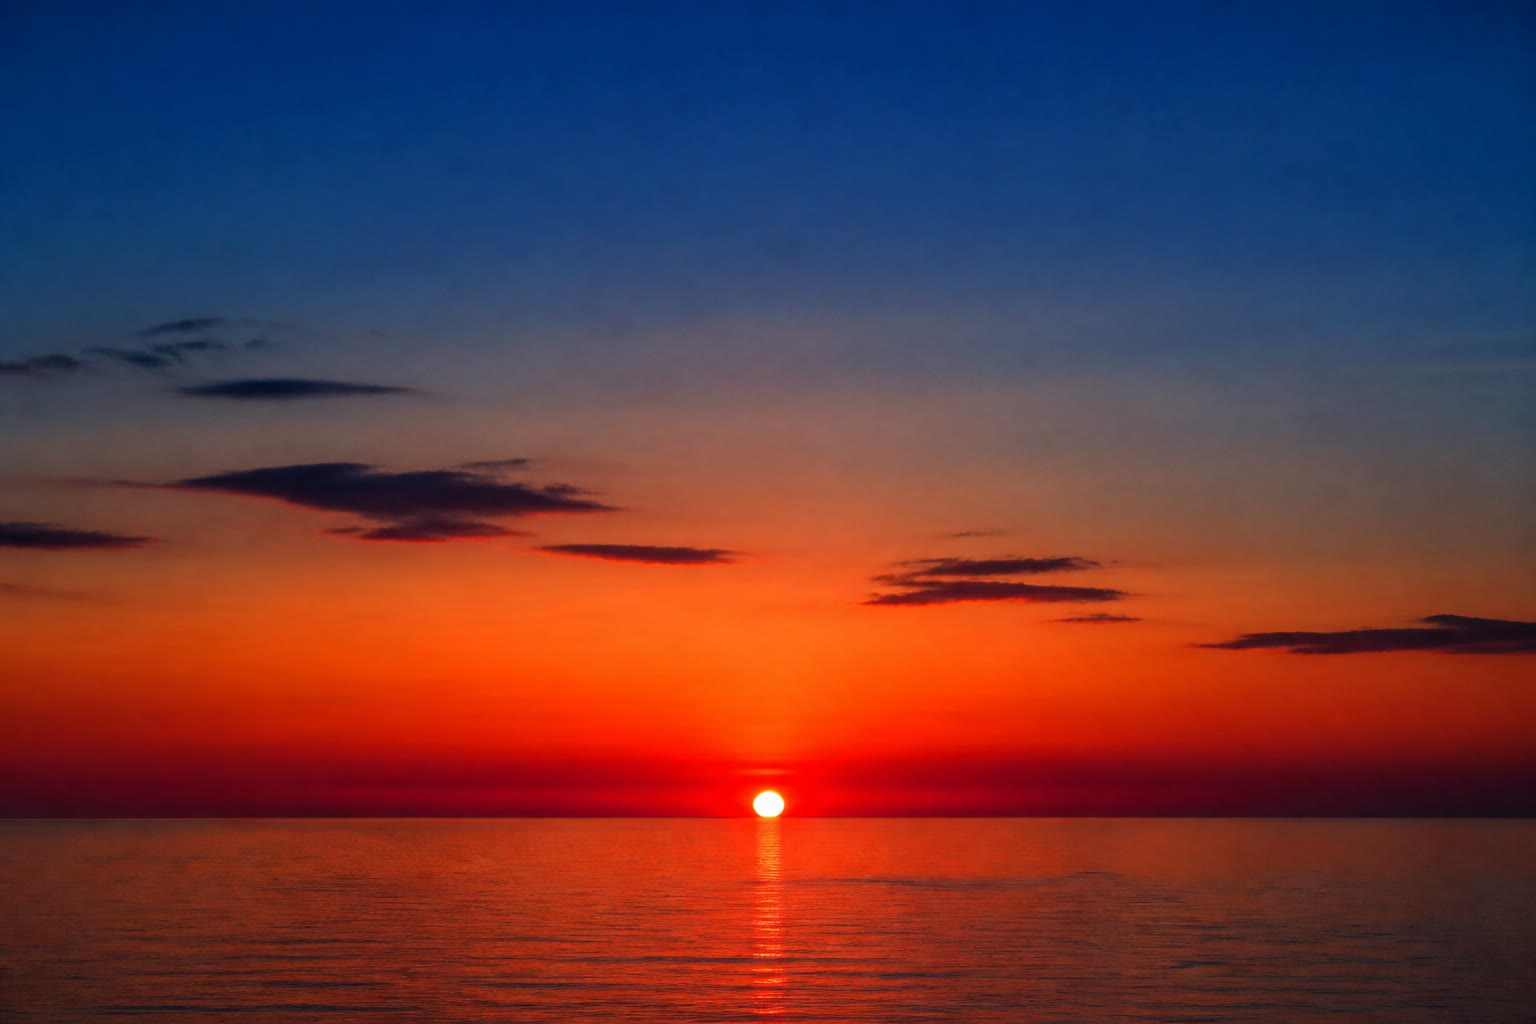
\includegraphics[width=0.58\linewidth]{images/book5/ai/b5-13-red-sunset.jpg}

{\small 日落即微扰论：空气分子对蓝光的散射远强于红光（本章黄金规则的同类，其中含 $\omega^4$ 因子），因此地平线处的长光程滤走蓝光，把它寄给了别处的正午天空。}
\end{omfigure}

\section{练习}

\begin{exercise}[$\star$]\label{exo:b3:perturbation-theory:1}
位于势箱 $[0, a]$ 中的粒子受附加势 $V(x) =
\lambda x/a$。（a）求各能级的一阶移动
（在任一箱态中取 $\langle x\rangle = a/2$——并说明理由）。
（b）为何此处各能级的移动相同？（c）
\emph{能级间距}的一阶变化是什么，为何测量跃迁频率
可能完全察觉不到这一微扰？
（d）一阶微扰何时不再可靠？
\end{exercise}

\begin{exercise}[$\star$]\label{exo:b3:perturbation-theory:2}
完整进行
\cref{prop:b3:perturbation-theory:oscillator-field}的二阶计算，包括
$\hat x$ 的矩阵元、两项、$n$ 的相消，以及
与配方法的结果精确一致。为何
\emph{态}的一阶修正不为零，而
能量的一阶修正为零？
\end{exercise}

\begin{exercise}[$\star$]\label{exo:b3:perturbation-theory:3}
二能级\omterm{def:b3:hamiltonian-mechanics:hamiltonian}{哈密顿量} $\begin{pmatrix}E_1 & v\\ v &
E_2\end{pmatrix}$，$E_1 < E_2$，$v$ 为实数。（a）求精确
\omterm{def:b3:quantum-formalism:observable}{本征值}。（b）在 $|v| \ll E_2 - E_1$ 下展开，并辨认
二阶公式。（c）证明能级会相互排斥，间隙总是
大于 $E_2 - E_1$。（d）当 $E_1 = E_2$ 时，微扰论
给出什么，精确解又给出什么，本章哪条定理
使两者协调一致？
\end{exercise}

\begin{exercise}[$\star$]\label{exo:b3:perturbation-theory:4}
对 \cref{thm:b3:perturbation-theory:corrections}：（a）证明
一阶态修正与 $\ket n$ 正交；（b）证明
$\ket m$ 的混合系数为 $V_{mn}/(E_n - E_m)$，并
给出有效性判据；（c）某能级与其最近邻能级的间距为 $\qty{1}{eV}$，
二者以 \qty{0.1}{eV} 耦合，估计
混入概率；（d）间隙为 \qty{10}{meV} 时重做——
此时应改用何种方法替代该展开？
\end{exercise}

\begin{exercise}[$\star\star$]\label{exo:b3:perturbation-theory:5}
非谐键。在谐振子中加入 $\hat V = \beta\hat x^3 + \gamma\hat x^4$，
（a）证明 $x^3$ 项在一阶时不移动任何能级（
由宇称可知）。（b）证明 $x^4$ 项给出 $\Delta E_n =
3\gamma(\hbar/2m\omega)^2(2n^2 + 2n + 1)$（将 $\hat x^4$ 用
\omterm{def:b3:harmonic-oscillator:ladder}{升降算符}展开，只保留“平衡”项）。（c）对真实键，有效 $\gamma$ 为负（势阱
向外变软）：证明此时能级间距随
$n$ 增大而\emph{减小}。
（d）此结果可再现分子光谱中的哪一已观测特征
（见\cref{exo:b3:harmonic-oscillator:4}）？
\end{exercise}

\begin{exercise}[$\star\star$]\label{exo:b3:perturbation-theory:6}
在方形二维势箱中，简并对 $\ket{1,2},
\ket{2,1}$ 受微扰 $\hat V = \lambda\,xy$。（a）说明为何
非简并理论失效。（b）计算 $2\times2$ 矩阵，
即 $\hat V$ 在该对中的矩阵（积分可分解；$\int_0^a
x\sin(\pi x/a)\sin(2\pi x/a)\dd x = -8a^2/9\pi^2$）。（c）求
劈裂及正确的零级态。（d）与
\cref{exo:b3:quantum-formalism:9}的对称性分析相比较：
对称性不费力即得出了哪一答案？
\end{exercise}

\begin{exercise}[$\star\star$]\label{exo:b3:perturbation-theory:7}
\omterm{ex:b3:perturbation-theory:stark}{斯塔克效应}，线性与二次。（a）利用
\cref{ex:b3:perturbation-theory:stark}，计算 $n = 2$
在 $\mathcal E = \qty{2.5e6}{V/m}$ 下的劈裂。（b）为何基态
\emph{不}出现线性移动（两个理由：宇称，以及
无简并伙伴）？（c）其二次移动定义了
极化率 $\Delta E = -\tfrac12\alpha\mathcal E^2$：估计
$\alpha \sim e^2a_0^2/E_{\text{I}}$，并以
$a_0^3$ 为单位求值（精确结果为 $4.5\,a_0^3 \times
4\pi\varepsilon_0$）。（d）物质的哪一日常性质——
即其介电响应——你刚刚算出的正是其
原子层面的根源？
\end{exercise}

\begin{exercise}[$\star\star$]\label{exo:b3:perturbation-theory:8}
自发辐射（承认一条输入）：激发态
以 $A = \omega^3|d_{fi}|^2/3\pi\varepsilon_0\hbar c^3$ 衰变，
其中偶极矩由 $d_{fi} = e\bra f\hat z\ket i$ 型矩阵元给出。
（a）对氢原子 $2p \to 1s$，取 $|d| \approx 0.74\,
ea_0$，$\lambda = \qty{121.6}{nm}$，计算 $A$ 与
寿命。（b）将结果推广到钠的 D 线。（c）推广到
超精细 21 厘米跃迁（$|d| \to$ 磁矩，速率
再降低约 $\alpha^2$ 量级的因子；取 $A \approx
\qty{2.9e-15}{s^{-1}}$）：检验“一千万年”的说法。（d）
由 $\omega^3$ 可知：为何紫外谱线衰变快，射电谱线
近乎永久，而这使得 21 厘米谱线
\emph{可预言}，却在实验室中几乎无法探测？
\end{exercise}

\begin{exercise}[$\star\star$]\label{exo:b3:perturbation-theory:9}
作为积分的选择定则。（a）由宇称证明 $\bra{100}\hat z\ket{200} =
0$。（b）证明 $\bra{100}\hat z\ket{21m} = 0$，除非 $m =
0$（$\varphi$ 积分）。（c）给出由此得到的规则 $\Delta
l = \pm1$，$\Delta m = 0, \pm1$，并说明其物理含义（
光子的自旋）。（d）$2s$ 态无法通过任何偶极途径跃迁至 $1s$
：这对其寿命有何预言，而自然界实际采取的
“禁戒”双光子路径是什么？
\end{exercise}

\begin{exercise}[$\star\star\star$]\label{exo:b3:perturbation-theory:10}
极化率的严格计算。氢原子
基态在电场中的二阶移动为 $\Delta E = -e^2\mathcal E^2\sum_{m\neq
0}|\bra m\hat z\ket 0|^2/(E_m - E_0)$。（a）对该和式作上界估计：
将每个分母替换为最小能隙 $E_2 - E_1 =
\tfrac34 E_{\text{I}}$，并利用闭合关系 $\sum_m|\bra
m\hat z\ket0|^2 = \langle z^2\rangle_0 = a_0^2$：给出 $\alpha
\le \tfrac{16}3\,a_0^3$（取高斯式单位
$4\pi\varepsilon_0$）。（b）与精确值 $\tfrac92 a_0^3$ 比较。
（c）由 $\alpha$ 估计氢气的折射率
在大气密度下（$n - 1 \approx N\alpha/2\varepsilon_0
\cdot e^2\dots$——取 $n - 1 = N\alpha_{\text{SI}}/2
\varepsilon_0$），并与测得的 $\num{1.3e-4}$ 比较。（d）
（d）用一句话说明周末问题第二部分所依托的链条：原子 $\to$
极化率 $\to$ 折射。
\end{exercise}

\begin{exercise}[$\star\star\star$]\label{exo:b3:perturbation-theory:11}
避免交叉与慢扫描。一个两能级系统的裸能量
为 $\pm\lambda t$，在 $t = 0$ 处交叉，并由 $v$ 耦合。（a）
画出精确能级随 $t$ 的变化：能隙为
$2|v|$ 的避免交叉。（b）若扫描\emph{缓慢}，系统沿
下方曲线演化（绝热定理，承认）：它最终
处于何种状态？（c）朗道–齐纳判据比较穿越能隙区域的扫描时间
$\sim v/\lambda$ 与内禀时钟
$\hbar/v$：给出绝热跟随的条件。（d）两种应用
：通过缓慢啁啾转移量子比特的态；原子碰撞中
电荷在原子核之间跃迁——用
两句话解释其中一种。
\end{exercise}

\begin{exercise}[$\star\star\star$]\label{exo:b3:perturbation-theory:12}
二阶是悲观主义者，以及其他定理。（a）证明
\emph{基态}的二阶修正总是
为负。（b）结合
\cref{exo:b3:harmonic-oscillator:10}，说明为何基态原子之间的范德瓦耳斯力
总是吸引的。（c）证明
一级理论\emph{高估}每个基态
能量：它是一个变分上界（计算 $\bra{\psi_0}\hat
H\ket{\psi_0}$，以未微扰态作为试探态）。（d）对
\cref{ex:b3:perturbation-theory:stark} 作一致性检验：为何
\emph{线性}\omterm{ex:b3:perturbation-theory:stark}{斯塔克效应}并不与（a）矛盾？
\end{exercise}

\section{问题：天空的颜色}

\begin{problem}[{周末问题——微扰原子的
瑞利散射}]\label{pb:b3:perturbation-theory:1}
白天的天空为何是蓝色的，日落时为何是红色的，而云是白色的？
完整答案是贯穿本章的一条链条：光波
使每个空气分子受到微扰；感应偶极子再次辐射（
即本科二年级分册中的偶极辐射）；而干涉决定
哪些成分得以保留。数据：空气分子的极化率
$\alpha/4\pi\varepsilon_0 \approx \qty{2.2e-30}{m^3}$；数
密度 $N = \qty{2.5e25}{m^{-3}}$；可见光范围
$450$--\qty{700}{nm}。

\medskip\noindent\textbf{第一部分——被微扰的分子。}
\begin{enumerate}
  \item 静电场 $\mathcal E$ 使分子的基态
        移动 $-\tfrac12\alpha\mathcal E^2$：将此结论与
        二阶\omterm{thm:b3:perturbation-theory:corrections}{微扰理论}联系起来（用哪个
        公式，为何为负？）。
  \item 同一 $\alpha$ 给出感应偶极矩 $p =
        \alpha\mathcal E$：对于太阳光的场 $\mathcal E \sim
        \qty{800}{V/m}$，计算一个
        氮分子的感应偶极矩，并与 $ea_0$ 比较。
  \item 光学场（频率 $\num{5e14}$ Hz）为何可以
        用\emph{静态}极化率处理，对于
        电子跃迁位于
        紫外区的分子？（比较 $\hbar\omega$ 与能隙；这是
        黄金规则分母的远离共振极限
        。）
  \item 振荡偶极子 $p_0\cos\omega t$ 辐射的
        平均功率为 $P = p_0^2\omega^4/12\pi\varepsilon_0c^3$
        （本科二年级分册）。结合 $p_0 = \alpha\mathcal
        E_0$：散射功率如何依赖于 $\omega$，
        在照明固定时？
  \item 计算 \qty{450}{nm}
        与 \qty{700}{nm} 处的散射功率之比。
  \item 用一句话说明：为何天空是蓝色而非紫色
        （两个因素：太阳光谱向紫端下降，以及
        人眼的灵敏度）？
\end{enumerate}

\medskip\noindent\textbf{第二部分——从单个分子到
天空。}
\begin{enumerate}[resume]
  \item 由此得散射截面 $\sigma =
        \dfrac{8\pi}{3}\Big(\dfrac{\alpha}{4\pi\varepsilon_0}
        \Big)^2\dfrac{\omega^4}{c^4}$：验证其量纲，
        并计算其在 \qty{550}{nm} 处的值。
  \item 衰减长度为 $\ell = 1/N\sigma$，计算其
        在 \qty{550}{nm} 处的值，并与大气层厚度比较
        （按海平面密度计的等效厚度 $\sim\qty{8}{km}$
        ）。
  \item 比较 \qty{450}{nm} 与 \qty{700}{nm}，竖直照射的阳光中
        有多大比例被散射掉？（取 $1 -
        \eu^{-L/\ell}$，其中 $L = \qty{8}{km}$。）
  \item 日落时光程为原来的三十倍，重新计算
        蓝光的存留比例，并解释低空太阳的颜色——
        以及月食中使月球变红的光的
        颜色。
  \item 为何距太阳 $90^\circ$ 处的天光是\emph{偏振}的
        （回想偶极子的辐射图样：沿偶极子轴向
        没有辐射）？
  \item 据称蜜蜂与维京人曾借助这种
        偏振导航：阴天时偏振将发生什么变化，
        为什么？
\end{enumerate}

\medskip\noindent\textbf{第三部分——天空为何不
更亮。}
\begin{enumerate}[resume]
  \item 一个悖论：在完全均匀的介质中，相邻体积元的子波
        在侧向相互发生相消干涉，
        因而\emph{没有}任何光会散射（只剩折射
        仍然存在）。究竟是什么打破了空气的均匀性——
        即什么在随机分布？
  \item 理想气体的密度涨落使独立分子的散射
        强度\emph{相加}。请说明
        独立性（随机位置、波长量级的间距）为何消除了
        相消干涉。
  \item 利用 \qty{550}{nm} 处的 $\ell$，求
        晴天时一层大气散射掉的阳光占比——
        这一数值是否与日常所见天空相对太阳的
        亮度相符？
  \item 一个云滴（\qty{10}{\micro m}）约含 $\sim10^{12}$
        个分子位于一个波长范围之内，它们的子波
        \emph{相干}地相加。那么散射功率
        如何随分子数变化，以及为何 $\omega^4$
        的颜色选择性消失（所有波长都强烈散射），
        云呈现什么颜色？
  \item 牛奶、雾与白漆呈白色的原因相同：
        请给出一般规律——散射体相对 $\lambda$ 较小时
        会使光着色，散射体相对 $\lambda$ 较大时
        则使光变白。
  \item 临界乳光：液体的临界点附近
        （本科一年级分册中的相变章节，以及
        后文的\cref{ch:b3:phase-transitions}），密度涨落增大到光学尺度，
        流体变得乳白。请联系第 13 题。
\end{enumerate}

\medskip\noindent\textbf{第四部分——完整的因果链。}
\begin{enumerate}[resume]
  \item 前向散射的子波\emph{并不}相互抵消：它们
        与入射光束发生干涉，使其相位减慢——即
        折射率。利用 $n - 1 = N\alpha/2\varepsilon_0$
        （$\alpha$ 取国际单位制），计算空气的 $n - 1$，
        并与实测值 \num{2.9e-4} 比较。
  \item 一个常数 $\alpha$ 由二阶\omterm{thm:b3:perturbation-theory:corrections}{微扰理论}算得，
        因此同时决定了三种现象：
        请说出它们（静电场中的能级移动；天空的蓝色；
        空气中光的弯曲）。
  \item 臭氧吸收、气溶胶与多次散射
        使真实天空更复杂：请各指出一个可观测量
        （暮光的颜色；乳白色地平线；
        日落后天顶残余的亮度）。
  \item 没有大气的月球，白天天空为何呈\emph{黑色}
——而月面上的每张照片由此证实了关于我们的天空
        起源的什么？
  \item 火星白天的天空呈奶油糖色，而其日落却呈
        \emph{蓝色}：稀薄的大气散射很弱，而悬浮的
        微米尺度尘埃颗粒起主要作用。利用
        第 18 题的规律，说明尘埃如何颠倒了颜色的逻辑。
  \item 对于 X 射线，$\hbar\omega$ 远大于每一个分子
        跃迁能级：电子的响应如同自由电子，而
        散射（汤姆孙）失去了其 $\omega^4$ 依赖性。
        “天蓝色”机制在该区域会发生什么变化——
        以及为何这种平坦的响应恰好使 X 射线
        成为探测电子密度的理想探针？
  \item 概括这一命名结果：一个 $\qty{2.2e-30}{m^3}$ 的极化率
        平方后再乘以 $\omega^4$，在绿光中给出
        量级为 \qty{60}{km} 的散射长度，
——既足够长以使正午天空温和，又足够短以使日落泛红、
        天空呈蓝色，并具有
        由一片受迫偶极子形成的偏振图样。
\end{enumerate}
\end{problem}
